\chapter{Algorithme utilisé pour l'heuristique}

% ####################################################################################################

\section{Recherche d'une solution initiale}

\paragraph{}
L'algorithme de descente locale va effectuer des mutations à partir d'une solution initiale.
Cette solution initiale est obtenue selon l'algorithme suivant :

\begin{algorithm}[H] % here (h) forced
\begin{algorithmic}
\STATE \COMMENT{Étape 1 : Tri des jobs selon EDD}
\STATE job[] $ \leftarrow $ trier\_jobs\_selon\_EDD(instance)
\STATE \COMMENT{Étape 2 : Initialisation, création de la première tournée}
\STATE créer\_nouvelle\_tournée()
\STATE ajouter\_dans\_dernière\_tournée(job[$ 1 $])
\STATE \COMMENT{Étape 3 : Double simulation pour les autres jobs}
\FOR{$ j = 2 $ \TO $ n $}
\STATE retard\_insertion $ \leftarrow $ simuler\_insertion\_dans\_dernière\_tournée(job[$ j $])
\STATE retard\_création $ \leftarrow $ simuler\_création\_nouvelle\_tournée(job[$ j $])
\IF{retard\_création $ < $ retard\_insertion}
\STATE créer\_nouvelle\_tournée()
\ENDIF
\STATE ajouter\_dans\_dernière\_tournée(job[$ j $])
\ENDFOR
\RETURN solution\_initiale
\end{algorithmic}
\caption{\label{alg:solution-initiale}Recherche d'une solution initiale}
\end{algorithm}

\paragraph{}
Les jobs sont d'abord triés par date de livraison croissante (tri EDD).
Ensuite, les jobs sont considérés un à un dans cet ordre, est la meilleure de ces deux alternatives est choisie :
\begin{itemize}
\item Le job considéré est ajouté à la dernière tournée de livraison.
\item Le job considéré est inséré dans une nouvelle tournée de livraison.
\end{itemize}
\paragraph{}
L'algorithme de NEH est utilisé pour constituer les ordonnancements.
L'algorithme de recherche du plus proche voisin est utilisé pour constituer les tournées de livraison.

\paragraph{}
Cet algorithme est une optimisation d'un algorithme précédemment implémenté par les étudiants au cours du premier semestre,
à l'occasion du mini-projet GPF (Gestion de Production et des Flux).

% ####################################################################################################

\section{Voisinage d'une solution}

\paragraph{}
Dans toute solution, les jobs sont répartis dans différentes tournées de livraison.
En numérotant ces tournées dans l'ordre chronologique, il est possible d'utiliser un tableau d'entiers
pour associer un numéro de job et un numéro de tournée.

\begin{figure}[H] % here (h) forced
\centering
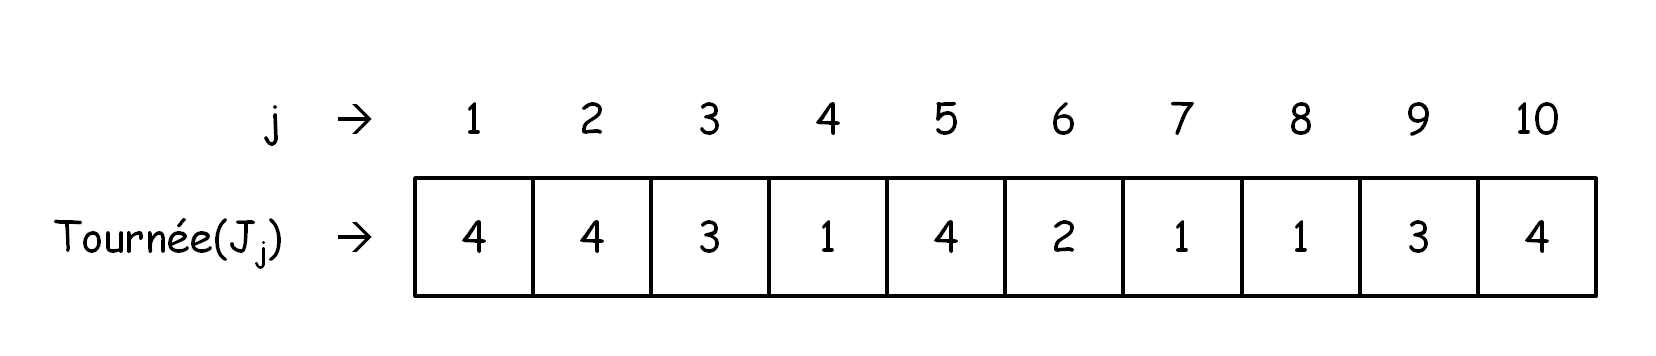
\includegraphics[scale=0.5]{association-job-tournee}
\caption{\label{fig:association-job-tournee}Représentation de l'affectation des jobs aux tournées de livraison}
\end{figure}

\paragraph{}
Dans cet exemple, les 10 jobs sont répartis dans les tournées suivantes :
\begin{enumerate}
\item Tournée de livraison 1 : jobs 4, 7 et 8 ;
\item Tournée de livraison 2 : job 6 ;
\item Tournée de livraison 3 : jobs 3 et 9 ;
\item Tournée de livraison 4 : jobs 1, 2, 5 et 10.
\end{enumerate}

\paragraph{Définition du voisinage d'une solution\\}
Étant donné une solution appelée \og solution mère \fg{}, le voisinage de cette solution est un ensemble de solutions,
appelées \og solutions filles \fg{}. La répartition des jobs en tournées de livraison pour ces solutions filles suit la règle suivante :
\begin{enumerate}
\item Tous les jobs \textit{sauf un} sont répartis dans les mêmes tournées de livraison que dans la solution mère.
\item Le \textit{job restant} est inséré dans une autre tournée : s'il appartenait à la tournée $ k $,
il appartient désormais soit à la tournée $ k - 1 $ (précédente), soit à la tournée $ k + 1 $ (suivante).
\end{enumerate}

\paragraph{Exemple\\}
Considérons la solution précédente comme solution mère. En diminuant le numéro de la tournée associée au job 5,
on obtient la solution fille suivante :

\begin{figure}[H] % here (h) forced
\centering
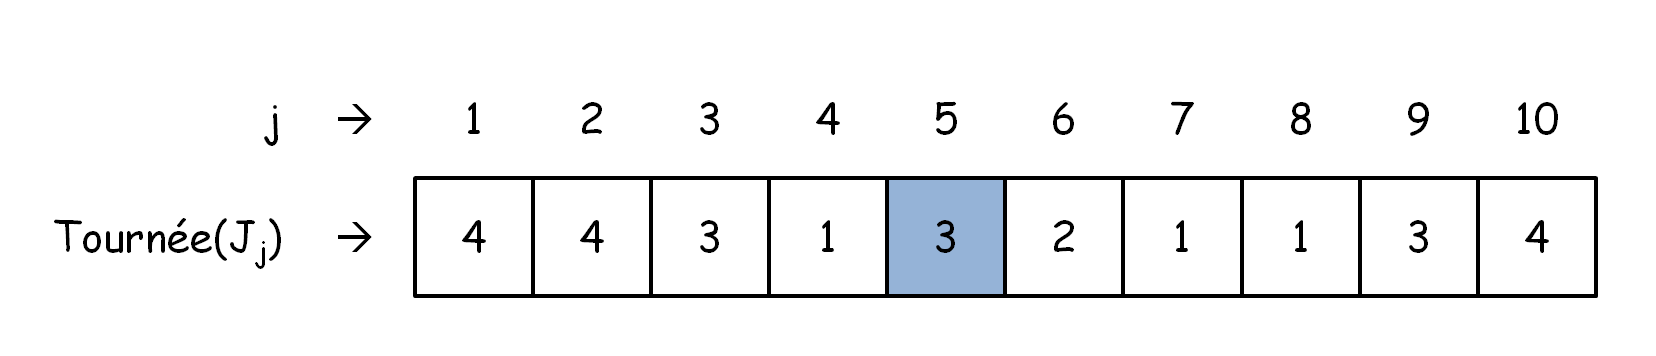
\includegraphics[scale=0.5]{voisinage-fille}
\caption{\label{fig:voisinage-fille}Exemple de solution fille}
\end{figure}

\paragraph{}
Dans cet exemple, les 10 jobs sont répartis dans les tournées suivantes :
\begin{enumerate}
\item Tournée de livraison 1 : jobs 4, 7 et 8 ;
\item Tournée de livraison 2 : job 6 ;
\item Tournée de livraison 3 : jobs 3, 5 et 9 ;
\item Tournée de livraison 4 : jobs 1, 2 et 10.
\end{enumerate}

% ####################################################################################################

\section{Descente locale}

\paragraph{}
L'algorithme utilisé est le suivant :

\begin{algorithm}[H] % here (h) forced
\begin{algorithmic}
\STATE solution\_mere $ \leftarrow $ trouver\_solution\_initiale(instance)
\STATE continuer $ \leftarrow $ \TRUE
\WHILE{continuer}
\STATE continuer $ \leftarrow $ \FALSE
\STATE \COMMENT{Génération de solutions filles}
\FOR{$ k = 1 $ \TO $ nombre\_mutations $}
\STATE solution\_fille[$ k $] $ \leftarrow $ générer\_mutation(solution\_mere)
\STATE \COMMENT{L'algorithme fait en sorte que toutes les solutions filles \\ soient différentes de la solution mère et des autres solutions filles.}
\ENDFOR
\STATE \COMMENT{Sélection de la meilleure solution fille}
\FOR{$ k = 1 $ \TO $ nombre\_mutations $}
\IF{somme\_retards(solution\_fille[$ k $]) $ < $ somme\_retards(solution\_mere)}
\STATE solution\_mere $ \leftarrow $ solution\_fille[$ k $]
\STATE continuer $ \leftarrow $ \TRUE { } \COMMENT{Effectuer une nouvelle itération}
\ENDIF
\ENDFOR
\ENDWHILE
\RETURN solution\_mere
\end{algorithmic}
\caption{\label{alg:heuristique}Algorithme de l'heuristique, descente locale à partir d'une solution initiale}
\end{algorithm}

\paragraph{}
À partir de la solution \og mère \fg{} initiale trouvée, certaines solutions \og filles \fg{} sont sélectionnées \textbf{aléatoirement} dans le voisinage.
Ce processus est appelée \og mutation \fg{}.
Si l'une des solutions filles est meilleure que la solution mère, elle devient la solution mère utilisée pour la prochaine itération.
L'algorithme continue jusqu'à ce que la solution mère soit meilleure ou équivalente à toutes ses filles (critère : somme des retards).

\paragraph{}
Le nombre de solutions filles considérées à chaque itération ($ nombre\_mutations $) est un paramètre optionnel de l'algorithme.
Si aucune valeur n'est spécifiée lors de l'invocation du programme, la valeur par défaut utilisée est égale au nombre de jobs dans l'instance.

\paragraph{Attention}
Le voisinage d'une solution est un ensemble de taille finie. Or, à chaque itération, l'algorithme fait en sorte de générer des solutions distinctes.
Par conséquent, si la valeur du paramètre $ nombre\_mutations $ est trop élevée, le programme tournera indéfiniment, car il restera bloqué
au niveau de la boucle de génération des solutions filles.
